\documentclass[11pt,a4paper]{article}
\usepackage[utf8]{inputenc}
\usepackage[T1]{fontenc}
\usepackage{geometry}
\geometry{a4paper, margin=1.0in}
\usepackage{hyperref}
\usepackage{graphicx}
\usepackage{titlesec}
\usepackage{parskip}
\usepackage{setspace}
\usepackage{listings}
\usepackage{xcolor}
\usepackage{longtable}
\usepackage{array}
\usepackage{float}

\definecolor{codegray}{rgb}{0.35,0.35,0.35}
\definecolor{backcolour}{rgb}{0.97,0.97,0.97}

\lstset{
    backgroundcolor=\color{backcolour},
    commentstyle=\color{codegray},
    basicstyle=\ttfamily\small,
    breaklines=true,
    captionpos=b,
    keepspaces=true,
    showspaces=false,
    showstringspaces=false,
}

\title{\textbf{FlexQL Database Engine}\\[0.4em]\Large Detailed Design and Architecture Document}
\author{}
\date{\today}

\begin{document}

\maketitle

\vspace{-1.2em}
\begin{center}
\renewcommand{\arraystretch}{1.25}
\begin{tabular}{rl}
\textbf{Name:} & \textbf{Nilesh Gupta} \\
\textbf{Roll No.:} & 25CS60R64 \\
\textbf{GitHub Repository:} & \href{https://github.com/Nilesh0711/FLEXQL}{github.com/Nilesh0711/FLEXQL} \\
\end{tabular}
\end{center}
\vspace{0.6em}

\begin{spacing}{1.08}

\begin{abstract}
FlexQL is a compact relational database engine implemented primarily in C with benchmark and test drivers in C++. The current system exposes a loopback-only client/server interface, persists table data on disk, maintains a per-table primary-key B+ tree index, replays a write-ahead log during startup, and uses an in-memory LRU cache for selected query results. This document describes the design as implemented in the repository, including the parser, executor, storage format, concurrency model, recovery path, query optimization choices, and operational limitations.
\end{abstract}

\tableofcontents
\newpage

\section{System Overview}

FlexQL is designed as a focused SQL execution engine rather than a full SQL database. The repository implements a narrow but coherent stack:

\begin{itemize}
    \item a public C API used by the REPL, tests, and benchmarks,
    \item a multithreaded TCP server bound to loopback,
    \item a handwritten SQL tokenizer and parser,
    \item an executor that chooses between index lookup, sequential scan, indexed join, and nested-loop join,
    \item a storage layer that persists schema metadata, row files, and primary-key index files,
    \item a small in-memory LRU cache for stable \texttt{SELECT} results,
    \item a simple write-ahead log used for crash recovery.
\end{itemize}

The system prioritizes:

\begin{itemize}
    \item simple persistence,
    \item predictable execution paths,
    \item moderate concurrency for concurrent readers,
    \item a clear, teachable implementation structure.
\end{itemize}

\section{Goals and Non-Goals}

\subsection{Goals}

\begin{itemize}
    \item Support a practical subset of SQL sufficient for table creation, insertion, selection, filtering, ordering, and joins.
    \item Persist all data on disk across process restarts.
    \item Speed up equality lookup on the first column of each table using a persisted B+ tree.
    \item Allow multiple client connections through a single server process.
    \item Recover from interrupted mutating statements using WAL replay on startup.
    \item Keep the codebase modular enough for coursework, experimentation, and benchmarking.
\end{itemize}

\subsection{Non-Goals}

\begin{itemize}
    \item Full SQL compliance.
    \item Distributed operation or remote host support.
    \item Transactions with commit/rollback semantics.
    \item Predicate-based row deletion or row updates.
    \item Secondary indexes, query planning statistics, or cost-based optimization.
    \item MVCC or fine-grained lock management.
\end{itemize}

\section{Supported SQL Surface}

The parser and executor currently recognize the following statement families:

\begin{longtable}{|>{\raggedright\arraybackslash}p{0.24\textwidth}|>{\raggedright\arraybackslash}p{0.68\textwidth}|}
\hline
\textbf{Statement} & \textbf{Behavior in Current Code} \\
\hline
\texttt{CREATE TABLE [IF NOT EXISTS] ...} & Creates metadata, row file, and primary-key index file. \\
\hline
\texttt{INSERT INTO ... VALUES (...), (...)} & Supports single-row and multi-row insertion. Values are validated against declared types before persistence. \\
\hline
\texttt{SELECT ... FROM ...} & Supports projection, \texttt{*}, optional \texttt{WHERE}, optional \texttt{INNER JOIN}, and optional \texttt{ORDER BY}. \\
\hline
\texttt{DELETE FROM table} & Clears all rows in the target table by truncating the row file and resetting the index. \\
\hline
\texttt{RESET table} & Alias for the same table-clear behavior as \texttt{DELETE FROM table}. \\
\hline
\end{longtable}

Supported predicate operators are:

\begin{itemize}
    \item \texttt{=}
    \item \texttt{!=}
    \item \texttt{<}
    \item \texttt{<=}
    \item \texttt{>}
    \item \texttt{>=}
\end{itemize}

Important behavioral rules:

\begin{itemize}
    \item The first column of every table is treated as the primary indexed lookup key.
    \item \texttt{ORDER BY} is valid only if the ordered column appears in the \texttt{SELECT} output list.
    \item If a table has a column named \texttt{EXPIRES\_AT}, rows with expired timestamps are skipped during reads.
    \item The server accepts only loopback hosts: \texttt{127.0.0.1} and \texttt{localhost}.
\end{itemize}

\section{High-Level Architecture}

\subsection{Module Map}

Figure~\ref{fig:system-architecture} is intended to hold the rendered Mermaid architecture diagram for the overall FlexQL system. Export your Mermaid diagram as a PNG or PDF and place it at:

\begin{itemize}
    \item \texttt{diagrams/system\_architecture.png}
\end{itemize}

\begin{figure}[H]
    \centering
    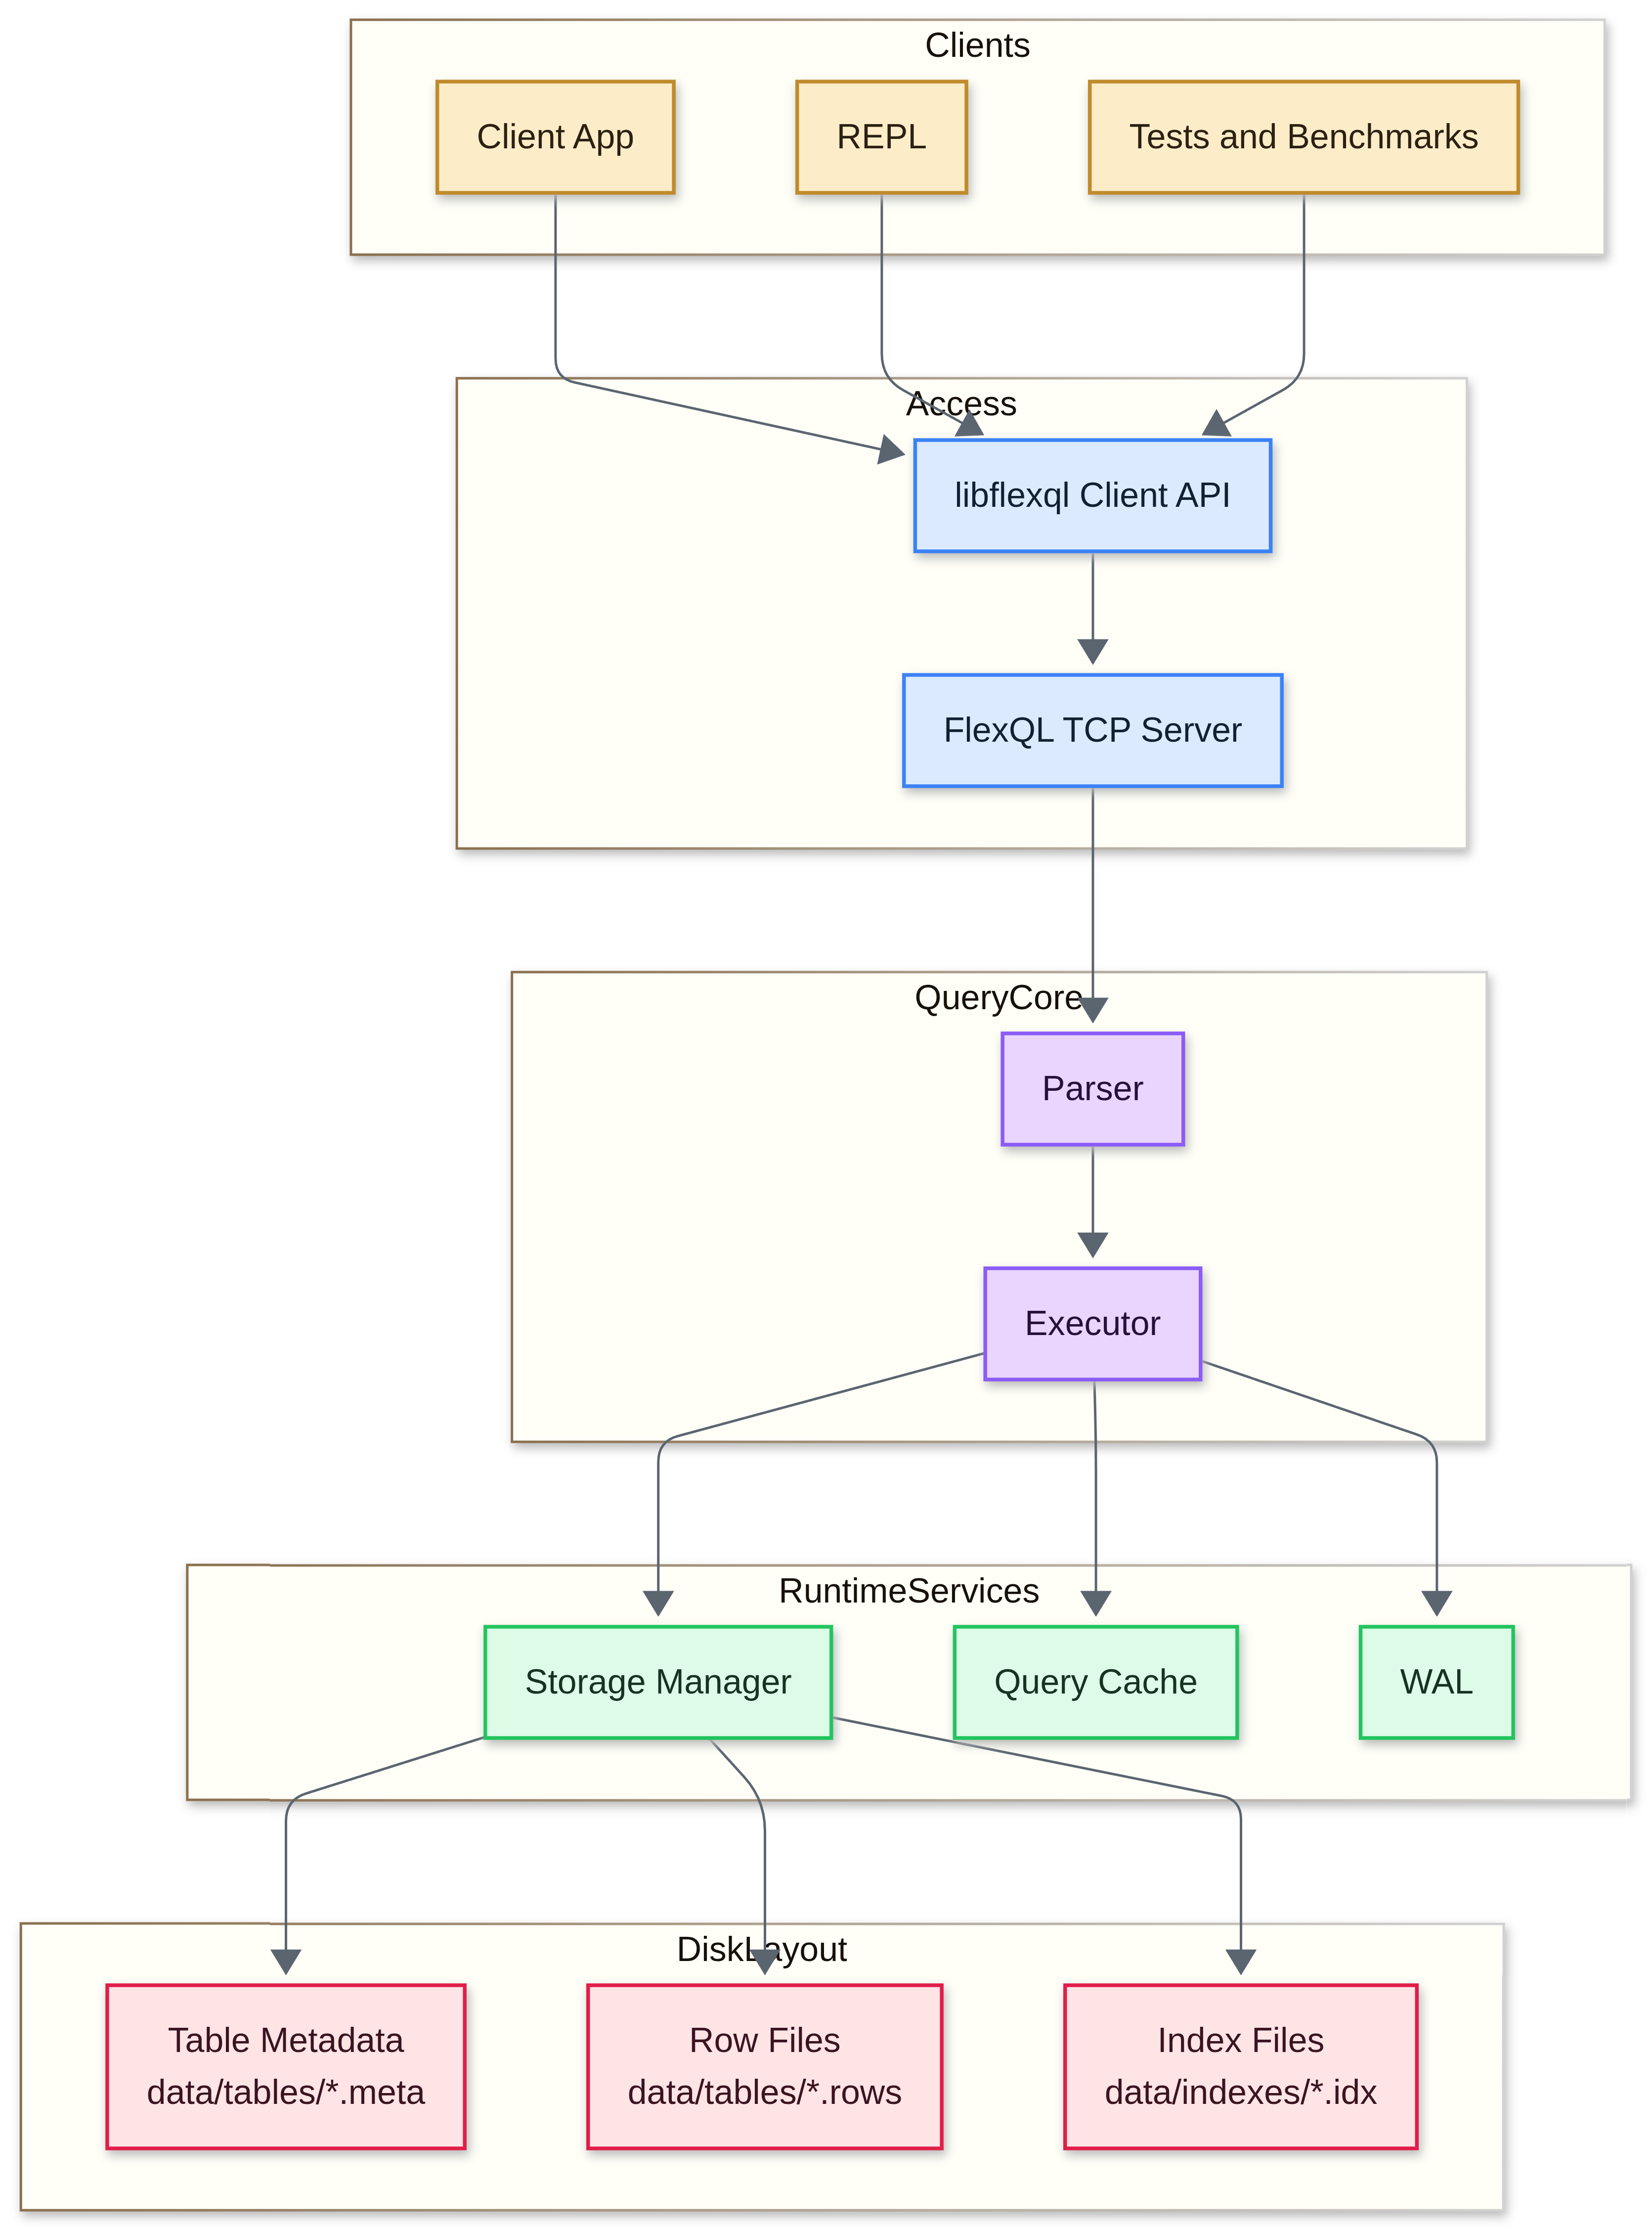
\includegraphics[width=0.8\textwidth]{diagrams/system_architecture.png}
    \caption{High-level FlexQL architecture showing client access, server runtime, parser, executor, and persistence subsystems.}
    \label{fig:system-architecture}
\end{figure}

For convenience, the Mermaid source that matches this section is:


\subsection{Runtime Components}

\begin{itemize}
    \item \textbf{Client API:} \texttt{flexql\_open}, \texttt{flexql\_exec}, \texttt{flexql\_close}, and \texttt{flexql\_free}.
    \item \textbf{Server runtime:} initializes storage and cache, replays the WAL, listens on a TCP port, and spawns one thread per accepted client connection.
    \item \textbf{Parser:} tokenizes SQL text and produces a statement structure.
    \item \textbf{Executor:} performs statement-specific work and decides whether to scan, sort, join, or use the primary index.
    \item \textbf{Storage manager:} owns table metadata in memory and file layout on disk.
    \item \textbf{Index manager:} persists and queries the B+ tree file for the first column of each table.
    \item \textbf{Cache:} stores recent \texttt{SELECT} results keyed by SQL text.
    \item \textbf{Expiration helper:} interprets \texttt{EXPIRES\_AT} as epoch time and suppresses expired rows at read time.
\end{itemize}

\section{Request Lifecycle}

\subsection{End-to-End Flow}

Figure~\ref{fig:request-lifecycle} is intended to hold the rendered Mermaid request-flow diagram. Export your Mermaid diagram as a PNG or PDF and place it at:

\begin{itemize}
    \item \texttt{diagrams/request\_lifecycle.png}
\end{itemize}

\begin{figure}[H]
    \centering
    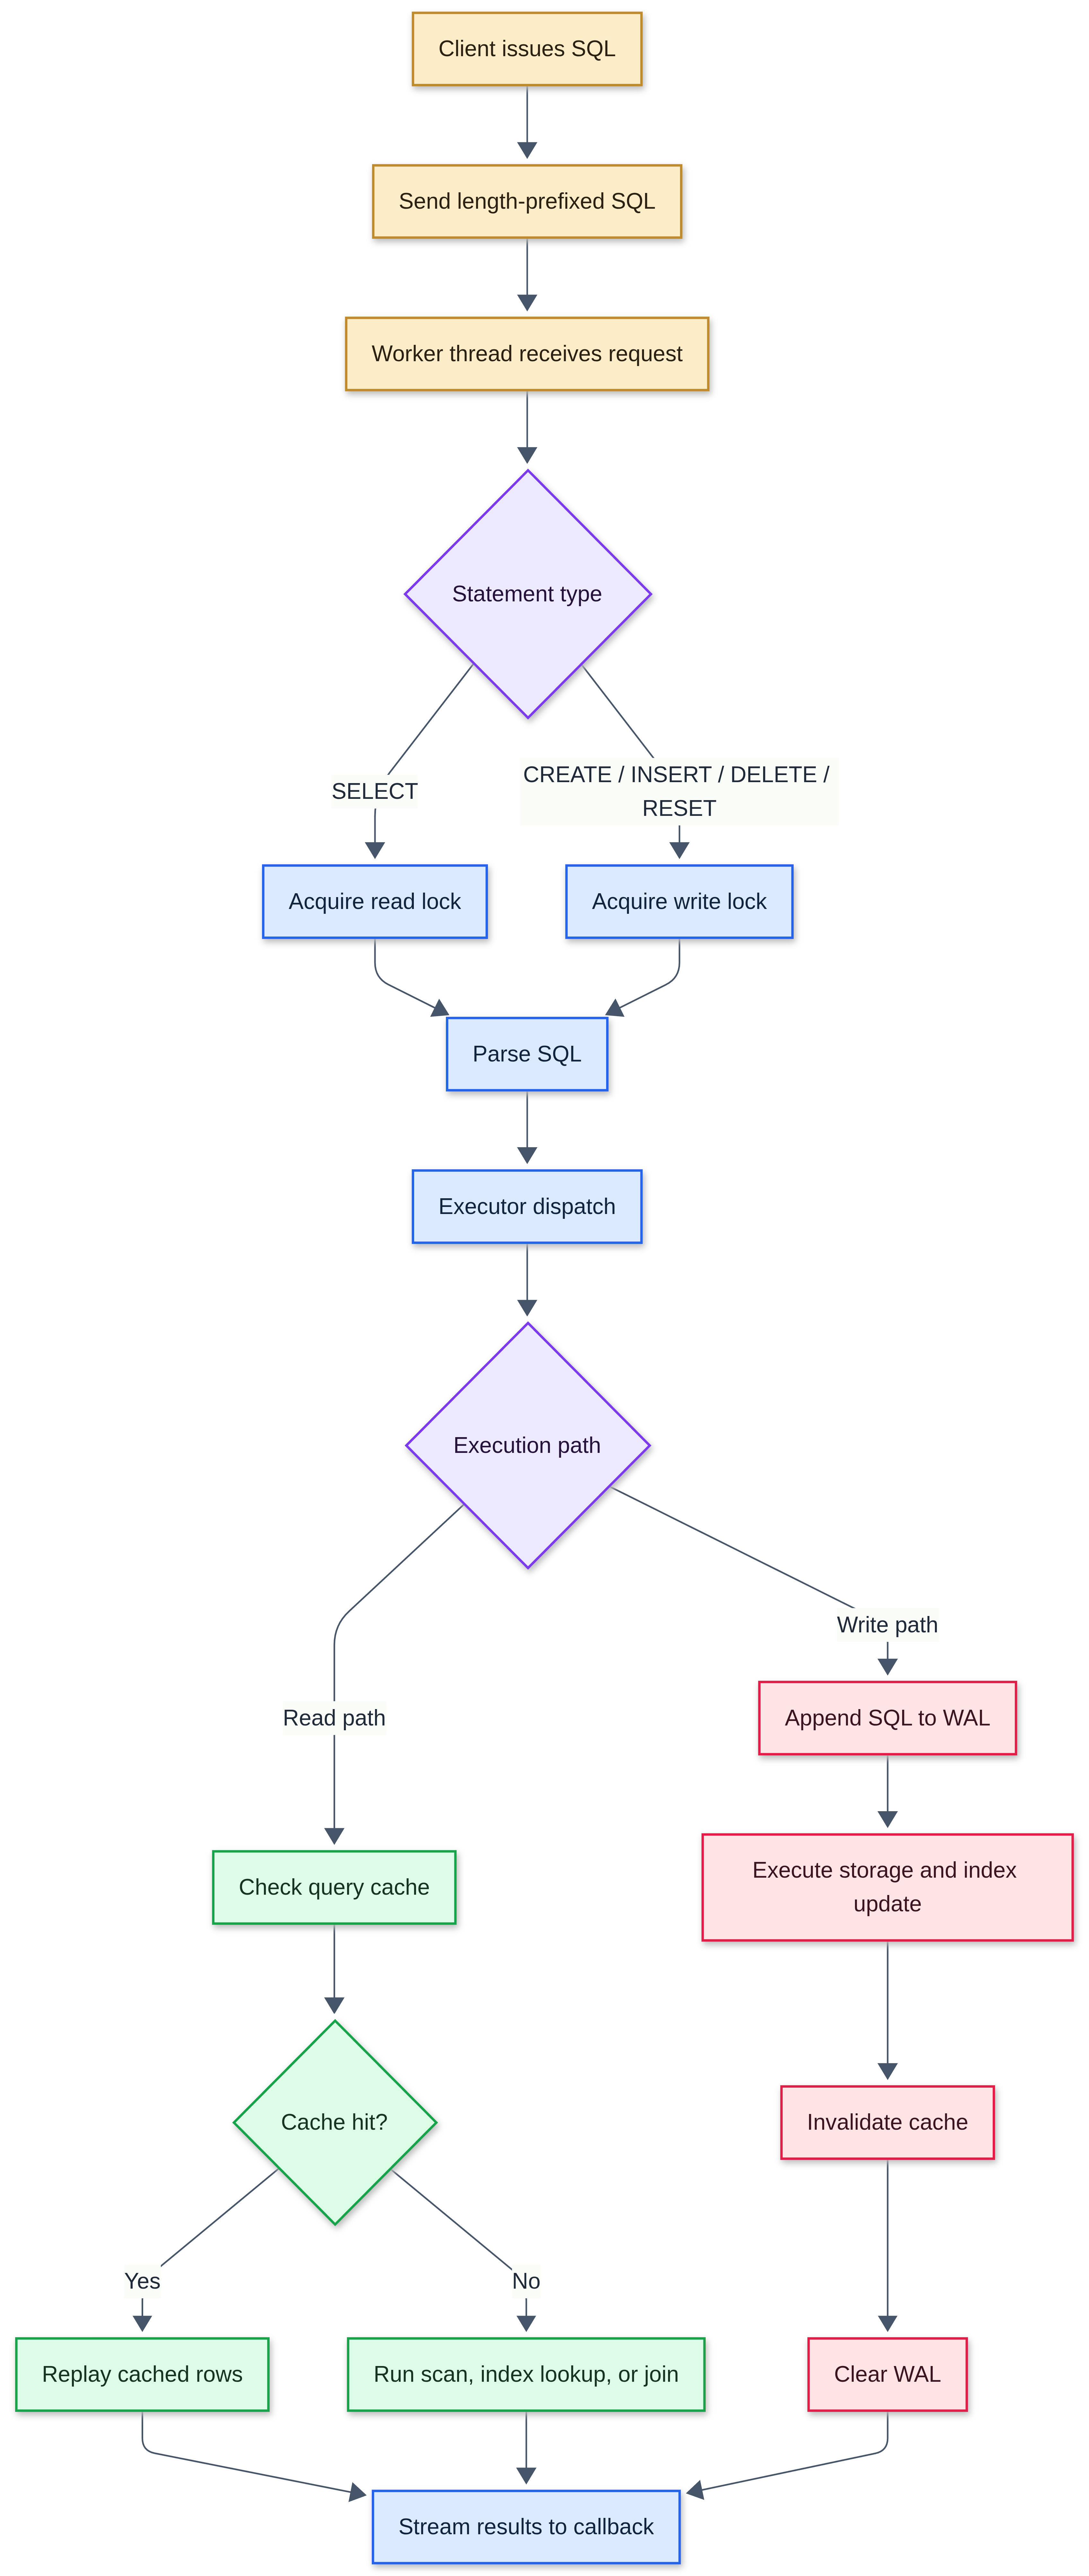
\includegraphics[width=0.5\textwidth]{diagrams/request_lifecycle.png}
    \caption{End-to-end request lifecycle from client SQL submission to streamed results.}
    \label{fig:request-lifecycle}
\end{figure}

\subsection{Client/Server Protocol}

The network protocol is intentionally simple and binary:

\begin{itemize}
    \item The client sends the SQL statement as \texttt{uint32 length + bytes}.
    \item The server streams results using markers and length-prefixed strings.
    \item Column names are sent once before row data.
    \item Each row is serialized column by column.
    \item Errors are sent as status markers plus an error string.
\end{itemize}

This protocol avoids text parsing on the wire and allows the server to stream large result sets without first rendering a textual table format.

\section{Parser Design}

\subsection{Tokenizer}

The parser uses a handwritten tokenizer in \texttt{src/parser/parser.c}. It recognizes:

\begin{itemize}
    \item identifiers and keywords,
    \item quoted string literals enclosed in single quotes,
    \item punctuation such as commas and parentheses,
    \item comparison operators such as \texttt{=}, \texttt{!=}, \texttt{<=}, \texttt{>=},
    \item statement terminators such as semicolons.
\end{itemize}

Each token stores:

\begin{itemize}
    \item token text,
    \item whether the token was quoted.
\end{itemize}

\subsection{Statement Structures}

The parser maps SQL into a tagged statement structure:

\begin{itemize}
    \item \texttt{FLEXQL\_STMT\_CREATE}
    \item \texttt{FLEXQL\_STMT\_INSERT}
    \item \texttt{FLEXQL\_STMT\_SELECT}
    \item \texttt{FLEXQL\_STMT\_DELETE}
    \item \texttt{FLEXQL\_STMT\_RESET}
\end{itemize}

For \texttt{SELECT}, the parser records:

\begin{itemize}
    \item whether \texttt{*} was used,
    \item projected columns,
    \item source table,
    \item join table and join condition if present,
    \item where condition if present,
    \item ordered column if present.
\end{itemize}

\subsection{Condition Representation}

Conditions are stored as:

\begin{itemize}
    \item left operand,
    \item comparison operator,
    \item right operand,
    \item whether the right operand was quoted,
    \item whether the right operand should be treated as a literal instead of a column reference.
\end{itemize}

This allows the executor to evaluate both:

\begin{itemize}
    \item literal predicates such as \texttt{ID = 2},
    \item column-vs-column predicates such as \texttt{TEST\_USERS.ID = TEST\_ORDERS.USER\_ID}.
\end{itemize}

\section{Execution Engine}

\subsection{Dispatcher}

Execution begins in \texttt{executor\_exec\_sql}. After parsing, the executor:

\begin{itemize}
    \item appends mutating statements to the WAL,
    \item dispatches by statement type,
    \item invalidates the cache after successful mutations,
    \item clears the WAL after successful completion.
\end{itemize}

\subsection{SELECT Execution Paths}

The most important implementation logic is in \texttt{execute\_select}. The executor chooses among several paths.

\subsubsection{Path 1: Cache Hit}

If the query is cacheable and an identical SQL string exists in the LRU cache, cached rows are replayed directly to the callback.

The query is \textbf{not} cached when any referenced table contains an \texttt{EXPIRES\_AT} column, because the visible rows depend on wall-clock time.

\subsubsection{Path 2: Primary-Key Equality Lookup}

For a single-table query of the form:

\begin{lstlisting}
SELECT ... FROM T WHERE first_column = literal;
\end{lstlisting}

the executor performs a direct index lookup using \texttt{storage\_lookup\_primary}. This turns a full scan into:

\begin{itemize}
    \item B+ tree lookup in \texttt{table.idx},
    \item row offset resolution,
    \item direct seek into \texttt{table.rows},
    \item deserialization of one row.
\end{itemize}

\subsubsection{Path 3: Sequential Scan}

All other single-table predicates are evaluated by scanning the row file using \texttt{storage\_scan\_open} and \texttt{storage\_scan\_next}. Each row is:

\begin{itemize}
    \item deserialized from the file stream,
    \item filtered for expiration if needed,
    \item tested against the \texttt{WHERE} clause,
    \item projected into the output row.
\end{itemize}

\subsubsection{Path 4: Indexed Join}

For \texttt{INNER JOIN} queries, the executor looks for a specific fast path:

\begin{itemize}
    \item the join operator must be \texttt{=},
    \item the join must compare columns from different tables,
    \item one side of the join condition must reference column index \texttt{0}.
\end{itemize}

When this holds, the executor scans one table and probes the other table through its primary index.

\begin{lstlisting}
scan non-indexed side -> read join key -> primary index lookup on other side
\end{lstlisting}

This is significantly cheaper than a full nested-loop join when the join predicate aligns with the indexed key.

\subsubsection{Path 5: Nested-Loop Join}

If the indexed join fast path does not apply, the executor performs:

\begin{itemize}
    \item an outer scan on the left table,
    \item an inner scan on the right table for every outer row,
    \item join condition evaluation for each row pair,
    \item optional post-join \texttt{WHERE} filtering.
\end{itemize}

\subsection{Projection Handling}

The executor resolves output columns before scanning data. It supports:

\begin{itemize}
    \item \texttt{SELECT *},
    \item unqualified column names when unambiguous,
    \item qualified names such as \texttt{TEST\_USERS.NAME}.
\end{itemize}

Each output column is converted into an internal reference identifying:

\begin{itemize}
    \item source table 1 or 2,
    \item column index within that table.
\end{itemize}

\subsection{Ordering}

\texttt{ORDER BY} is implemented by materializing result rows in memory and sorting them with a merge-sort style routine. Two design consequences follow:

\begin{itemize}
    \item ordered queries cannot stream rows immediately,
    \item the ordered column must be present in the output list.
\end{itemize}

When no ordering is requested and the query is not being cached, rows can be streamed directly to the callback.

\section{Storage Engine}

\subsection{Directory Layout}

The storage layer creates and uses:

\begin{itemize}
    \item \texttt{data/tables}
    \item \texttt{data/indexes}
    \item \texttt{data/wal}
\end{itemize}

Each table owns three logical artifacts:

\begin{itemize}
    \item \texttt{<table>.meta}
    \item \texttt{<table>.rows}
    \item \texttt{<table>.idx}
\end{itemize}

\subsection{Metadata File}

The metadata file begins with a magic string and then stores:

\begin{itemize}
    \item table name,
    \item column count,
    \item row count,
    \item expiration column index,
    \item one line per column with name and declared type.
\end{itemize}

This lets the server reconstruct the table catalog during startup without scanning row files.

\subsection{Row File Format}

Rows are serialized in a compact binary format:

\begin{lstlisting}
[field_count:uint32]
    repeated field_count times:
        [value_length:uint32][value_bytes]
\end{lstlisting}

The system stores all row values as strings on disk. Type information is enforced at insert time rather than encoded in a typed binary row layout.

\subsection{Insert Path}

On insert:

\begin{itemize}
    \item the target table is located in memory,
    \item the number of supplied values must match the column count,
    \item every supplied value is validated against the declared type,
    \item serialized row bytes are appended to the row file,
    \item the first column value and row offset are inserted into the index file,
    \item the metadata row count is updated and flushed.
\end{itemize}

\subsection{Scan Path}

Sequential scans use a buffered reader. The scan state owns:

\begin{itemize}
    \item file pointer,
    \item large read buffer,
    \item reusable row value array,
    \item reusable string buffer for field contents.
\end{itemize}

This design reduces allocation churn during full-table scans.

\section{Type System and Validation}

The storage layer enforces a small set of types:

\begin{itemize}
    \item \texttt{INT}
    \item \texttt{DECIMAL}
    \item \texttt{DATETIME}
    \item \texttt{VARCHAR(n)}
\end{itemize}

Validation rules:

\begin{itemize}
    \item \texttt{INT}: must parse as an integer-valued number.
    \item \texttt{DECIMAL}: must parse numerically.
    \item \texttt{DATETIME}: accepts either a numeric epoch or the textual shape \texttt{YYYY-MM-DD HH:MM:SS}.
    \item \texttt{VARCHAR(n)}: must not exceed the declared limit.
\end{itemize}

Even though values are stored as strings, type validation prevents obviously invalid inserts.

\section{Primary-Key Index Design}

\subsection{Index Role}

Every table automatically gets one persisted B+ tree index over the first declared column. There are no secondary indexes in the current implementation.

\subsection{Index File Structure}

The index file stores:

\begin{itemize}
    \item a file header with magic value, root page number, and next page number,
    \item fixed-size pages,
    \item leaf and internal nodes in B+ tree form.
\end{itemize}

The implementation uses:

\begin{itemize}
    \item fixed key size of 64 bytes,
    \item up to 31 keys per page,
    \item a page cache inside the index subsystem for recently touched pages.
\end{itemize}

\subsection{Lookup and Insert Behavior}

\begin{itemize}
    \item \textbf{Lookup:} traverse from root to leaf and return the row offset when the key exists.
    \item \textbf{Insert:} descend recursively, insert into a leaf, split when full, and propagate split keys upward.
    \item \textbf{Reset:} recreate or clear the logical contents of the index when a table is cleared.
\end{itemize}

\subsection{Index Diagram}

Figure~\ref{fig:index-structure} is intended to hold the rendered Mermaid index-structure diagram. Export your Mermaid diagram as a PNG or PDF and place it at:

\begin{itemize}
    \item \texttt{diagrams/index\_structure.png}
\end{itemize}

\begin{figure}[H]
    \centering
    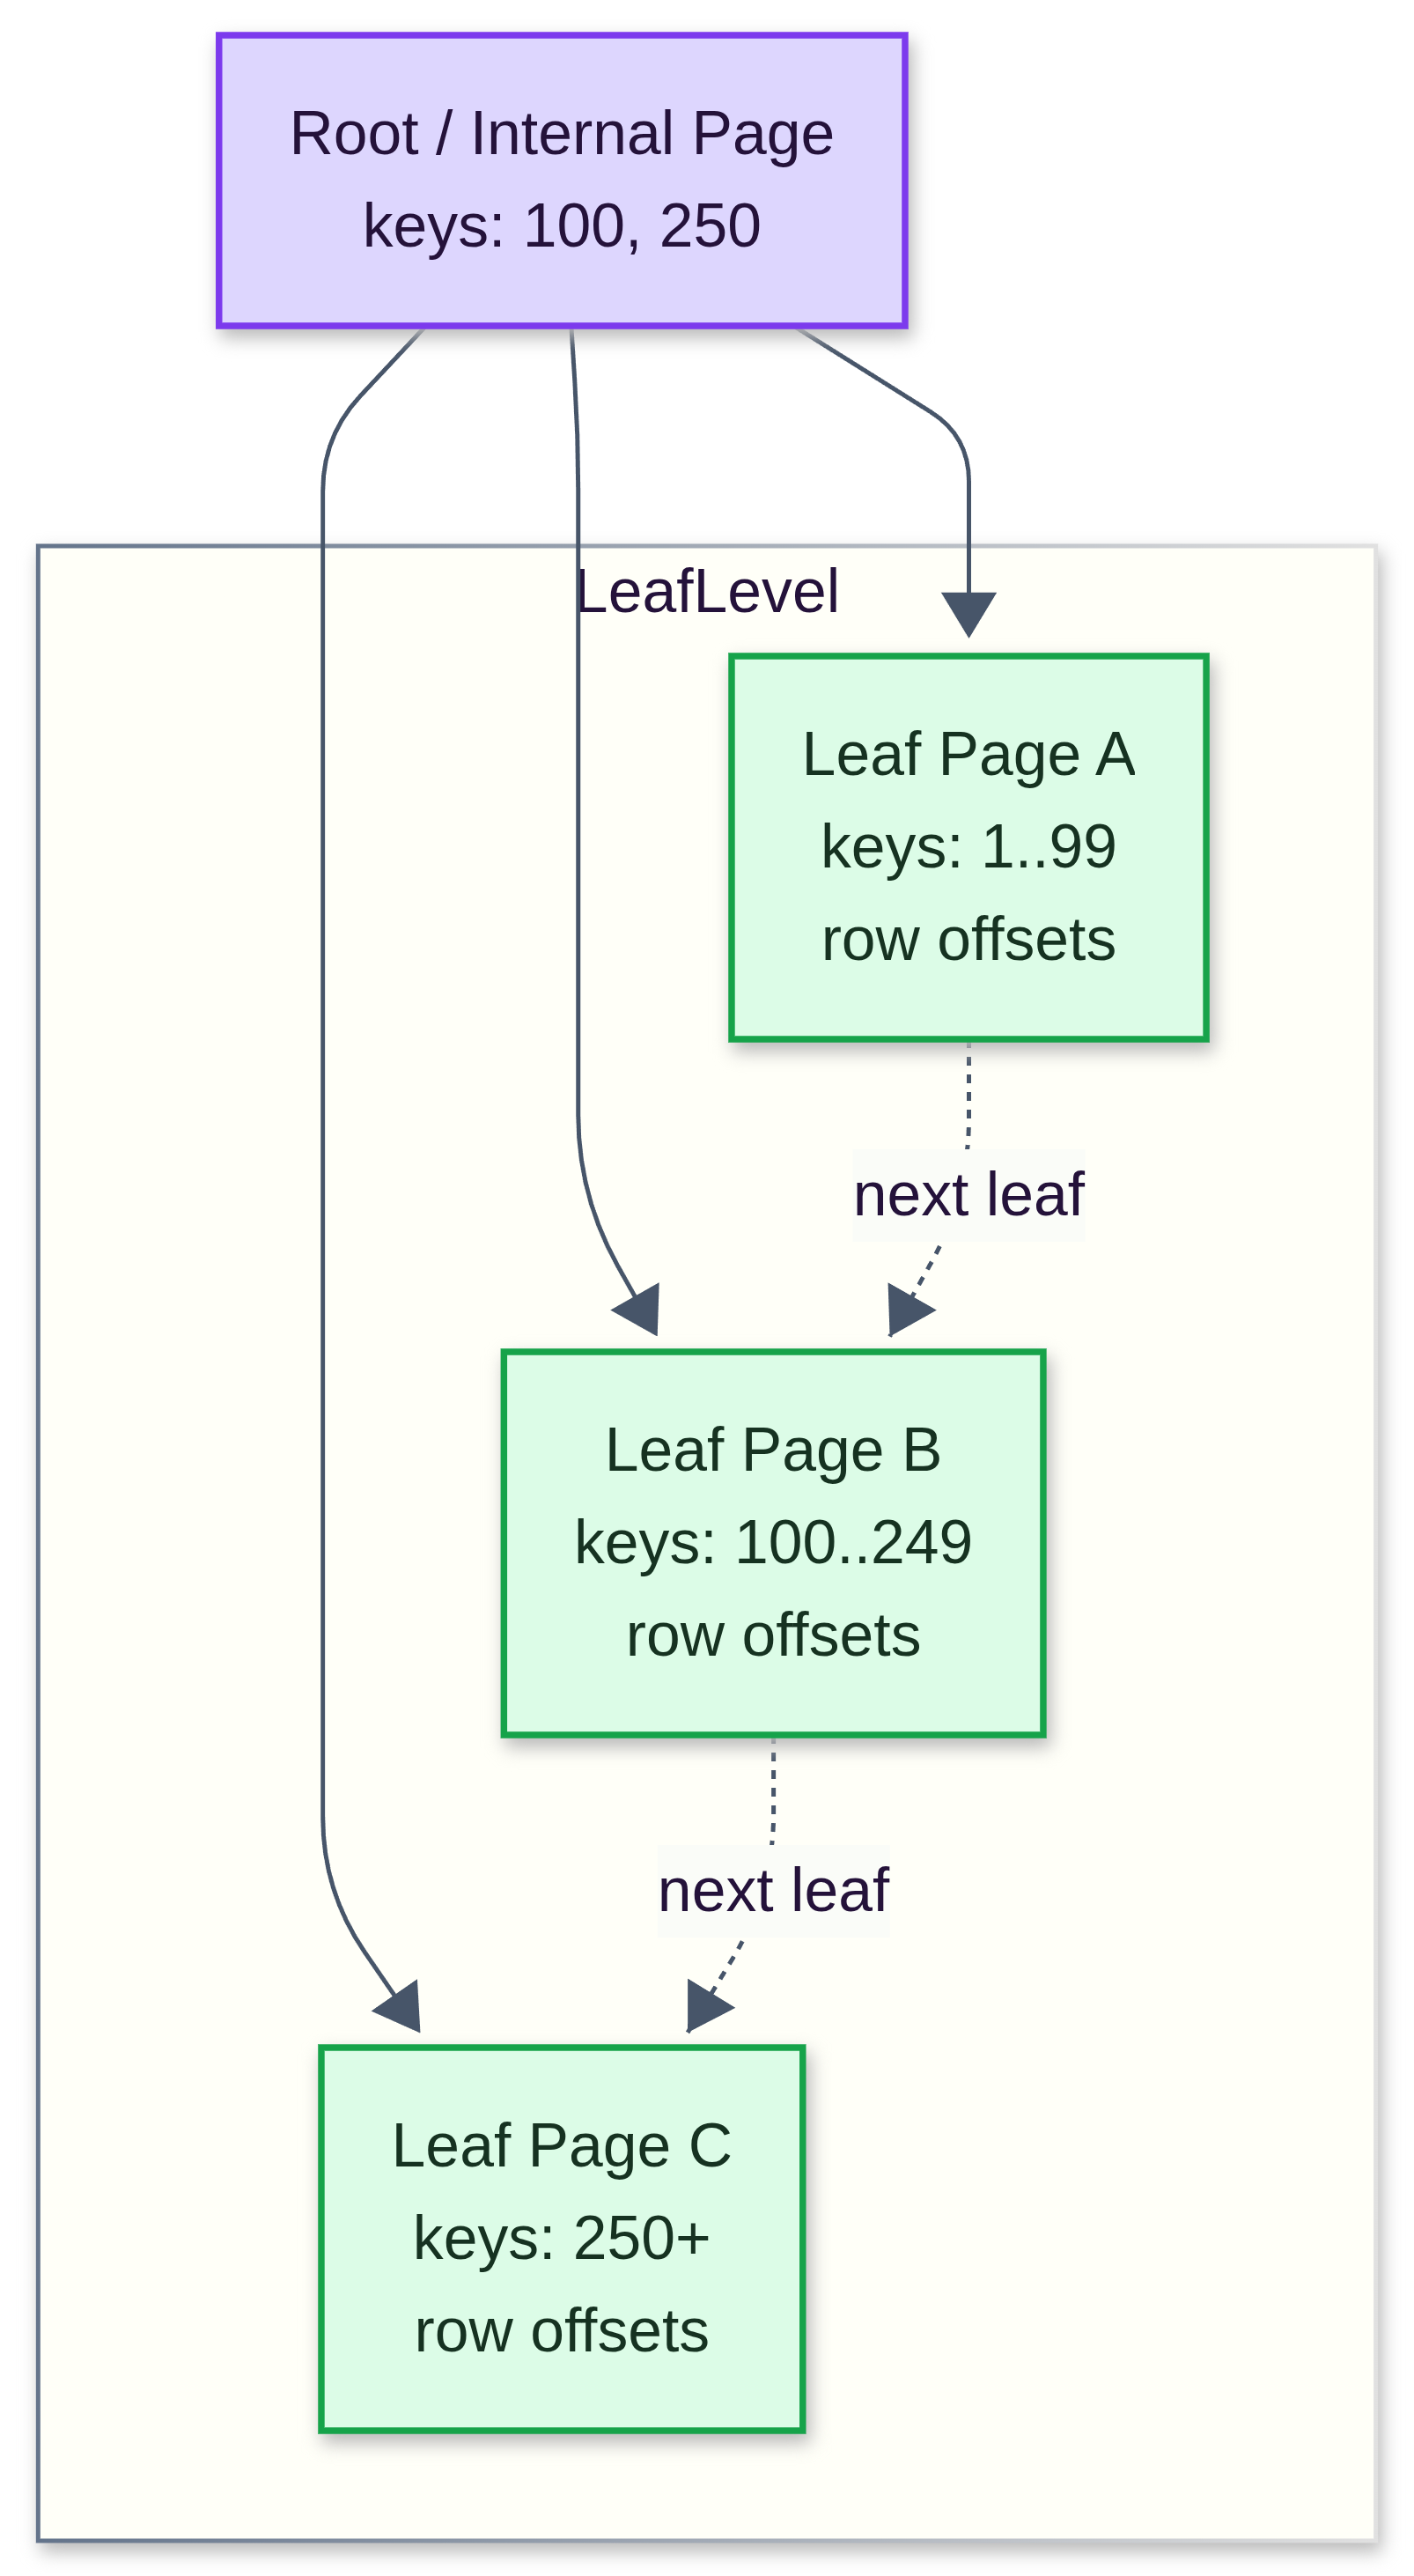
\includegraphics[width=0.5\textwidth]{diagrams/index_structure.png}
    \caption{Conceptual primary-key B+ tree layout used by FlexQL index files.}
    \label{fig:index-structure}
\end{figure}

\section{Caching Strategy}

\subsection{Purpose}

The query cache stores complete result sets for recently executed \texttt{SELECT} statements. The key is the literal SQL string.

\subsection{Structure}

Each cache entry contains:

\begin{itemize}
    \item SQL text,
    \item output column names,
    \item fully copied result rows,
    \item LRU tick,
    \item occupancy flag.
\end{itemize}

The server initializes the cache with capacity 16.

\subsection{Policy}

\begin{itemize}
    \item On a hit, the entry tick is refreshed.
    \item On insert into a full cache, the least-recently-used entry is replaced.
    \item On any successful mutating statement, the full cache is invalidated.
    \item Queries touching expiring rows are not cached.
\end{itemize}

\subsection{Tradeoff}

This cache is simple and effective for repeated identical reads, but it duplicates entire result sets in memory and does not support partial invalidation.

\section{Expiration Semantics}

If a column named \texttt{EXPIRES\_AT} exists, its column index is stored in table metadata. During reads:

\begin{itemize}
    \item the value is parsed as an epoch timestamp,
    \item rows with \texttt{EXPIRES\_AT < now()} are skipped,
    \item expired rows remain on disk and in the index until the table is cleared.
\end{itemize}

This is a read-time visibility rule, not a background garbage collection mechanism.

\section{Write-Ahead Logging and Recovery}

\subsection{WAL Format}

The WAL file is stored at \texttt{data/wal/flexql.wal}. Each record is:

\begin{lstlisting}
[sql_length:uint32][sql_bytes]
\end{lstlisting}

\subsection{When WAL Is Used}

The executor writes to the WAL before:

\begin{itemize}
    \item \texttt{CREATE TABLE}
    \item \texttt{INSERT}
    \item \texttt{DELETE FROM table}
    \item \texttt{RESET table}
\end{itemize}

Pure reads do not touch the WAL.

\subsection{Recovery Process}

At server startup:

\begin{itemize}
    \item storage and cache are initialized,
    \item the WAL file is opened,
    \item each stored SQL statement is replayed through the executor in recovery mode,
    \item the WAL is cleared after successful replay.
\end{itemize}

\subsection{Recovery Diagram}

Figure~\ref{fig:wal-recovery} is intended to hold the rendered Mermaid WAL recovery diagram. Export your Mermaid diagram as a PNG or PDF and place it at:

\begin{itemize}
    \item \texttt{diagrams/wal\_recovery.png}
\end{itemize}

\begin{figure}[H]
    \centering
    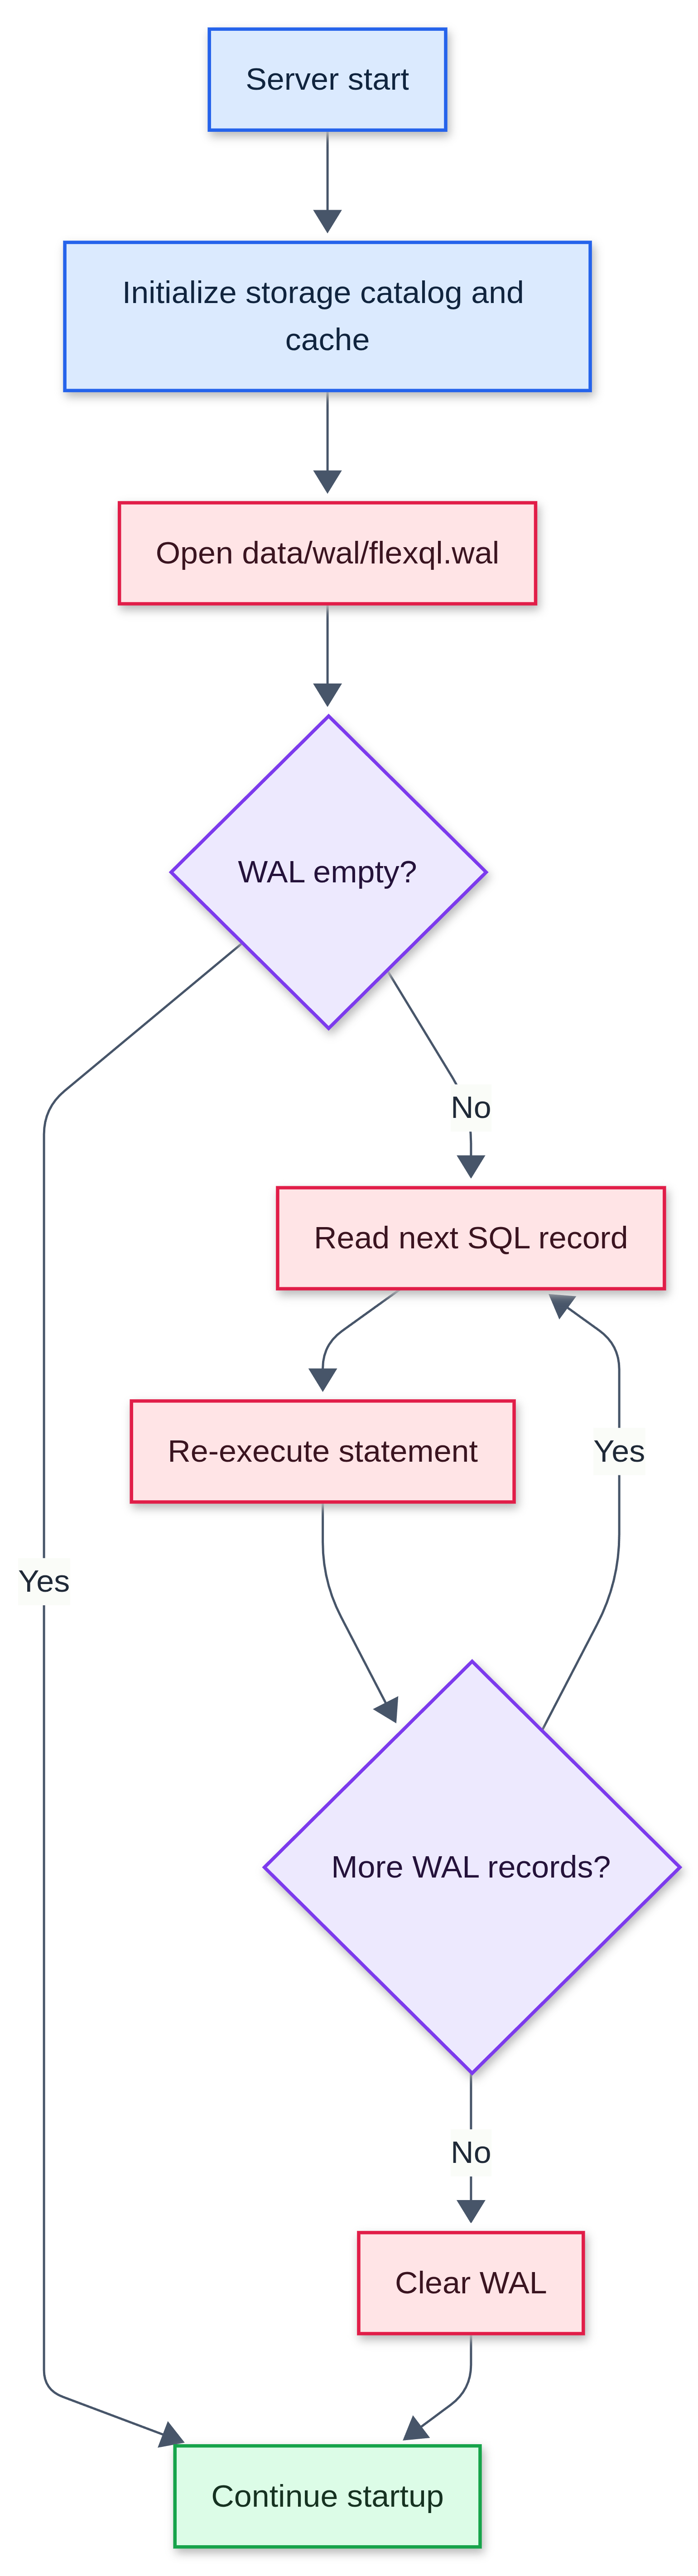
\includegraphics[width=0.3\textwidth]{diagrams/wal_recovery.png}
    \caption{Startup recovery flow using the write-ahead log.}
    \label{fig:wal-recovery}
\end{figure}

\section{Concurrency Model}

\subsection{Server Concurrency}

The server follows a thread-per-connection model:

\begin{itemize}
    \item the accept loop listens on a single socket,
    \item each accepted client is handed to a detached worker thread,
    \item every worker receives SQL requests in a loop until disconnect.
\end{itemize}

\subsection{Locking Policy}

The server owns one process-wide reader/writer lock for database operations:

\begin{itemize}
    \item \textbf{read lock} for statements whose first token is \texttt{SELECT},
    \item \textbf{write lock} for all other statements.
\end{itemize}

This means:

\begin{itemize}
    \item multiple readers can execute concurrently,
    \item writers are serialized,
    \item reads and writes do not overlap.
\end{itemize}

\subsection{Cache Synchronization}

The cache has its own mutex, because worker threads may read or update cache entries concurrently while still respecting the outer database lock policy.

\subsection{Concurrency Diagram}

Figure~\ref{fig:concurrency-model} is intended to hold the rendered Mermaid concurrency diagram. Export your Mermaid diagram as a PNG or PDF and place it at:

\begin{itemize}
    \item \texttt{diagrams/concurrency\_model.png}
\end{itemize}

\begin{figure}[H]
    \centering
    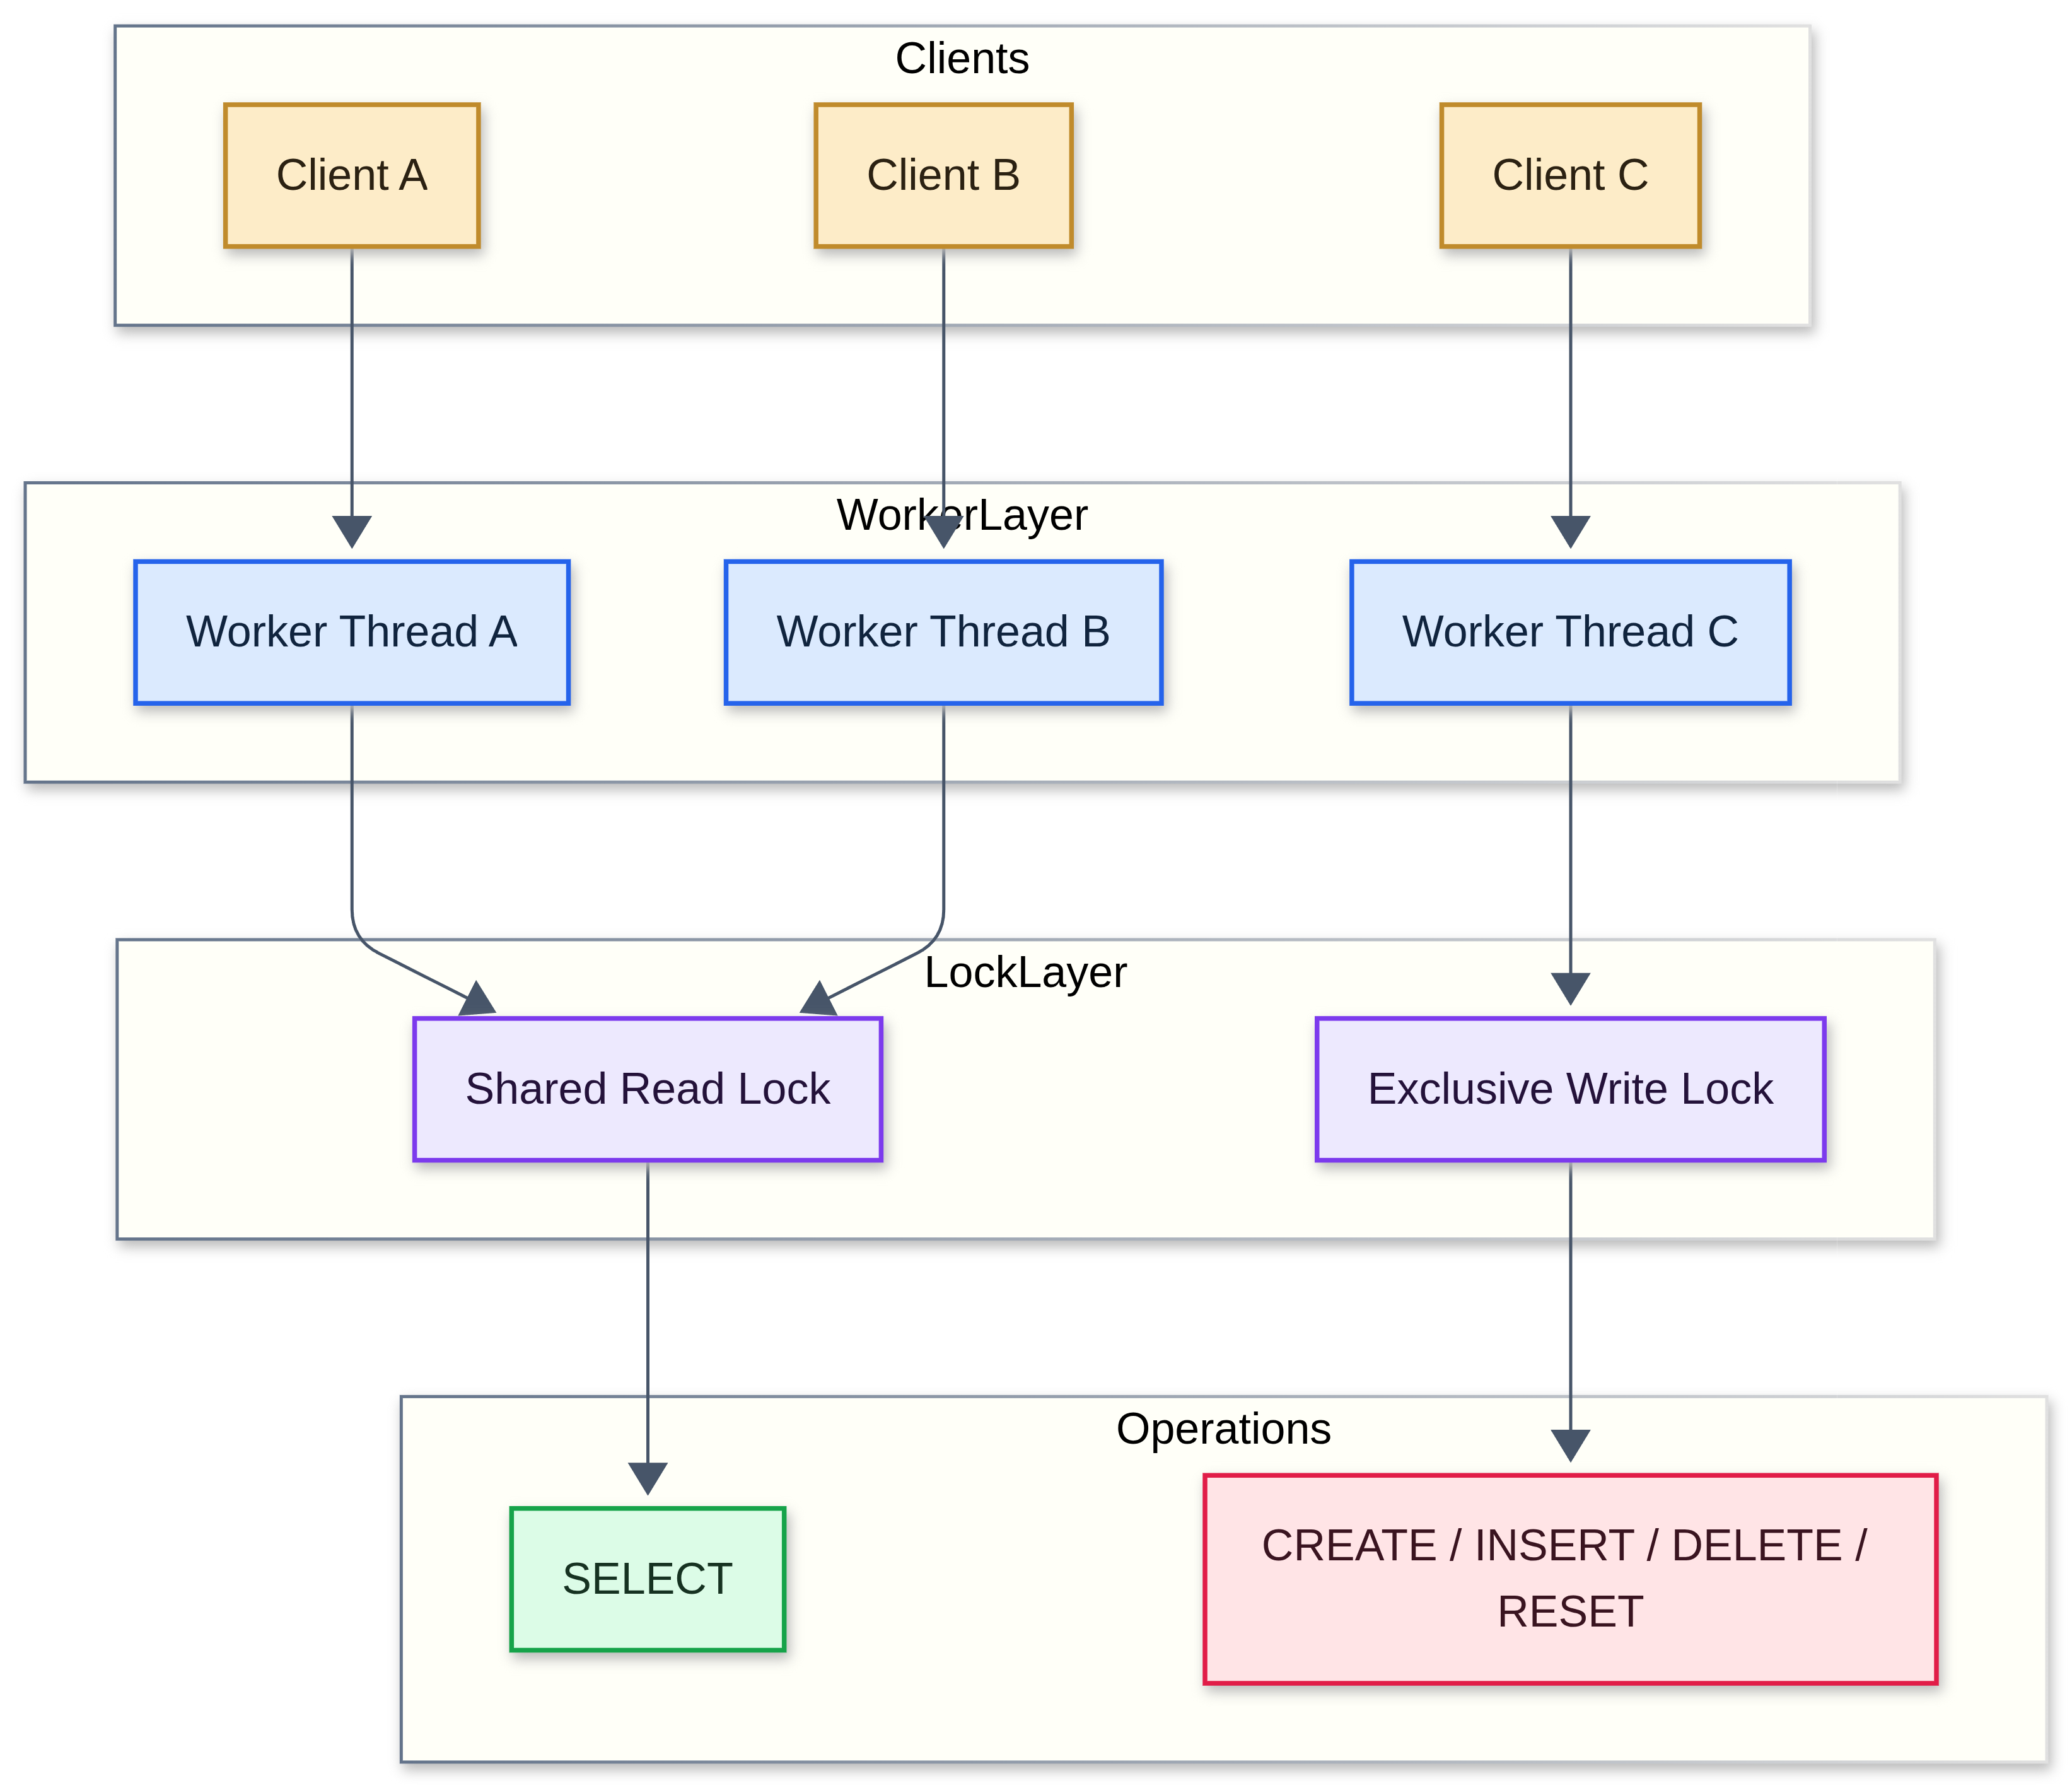
\includegraphics[width=\textwidth]{diagrams/concurrency_model.png}
    \caption{Thread-per-connection server model with shared read access and serialized writes.}
    \label{fig:concurrency-model}
\end{figure}

\section{Server and Client API}

\subsection{Public API}

The public API is intentionally small:

\begin{lstlisting}[language=C]
int flexql_open(const char* host, int port, flexql** db);
int flexql_close(flexql* db);
int flexql_exec(flexql* db, const char* sql,
                flexql_callback callback, void* arg, char** errmsg);
void flexql_free(void* ptr);
\end{lstlisting}

\subsection{Behavior}

\begin{itemize}
    \item \texttt{flexql\_open} validates the endpoint and opens a TCP connection.
    \item \texttt{flexql\_exec} sends SQL to the server and routes result rows through the callback.
    \item \texttt{flexql\_close} closes the connection and frees client-side resources.
    \item \texttt{flexql\_free} releases error strings returned to the caller.
\end{itemize}

The current user-facing path is remote execution through the local server. The internal handle contains fields for a local mode, but the normal public workflow in this repository is the TCP client/server path.

\section{Testing and Benchmarking}

\subsection{Regression Test Driver}

\texttt{tests/test\_driver.c} validates:

\begin{itemize}
    \item table creation,
    \item insertion,
    \item equality lookup on the primary key,
    \item range predicates and filtered scans,
    \item joins,
    \item ordering constraints,
    \item error behavior for unknown columns and invalid \texttt{ORDER BY}.
\end{itemize}

\subsection{Benchmarks}

The repository also includes benchmark programs that exercise:

\begin{itemize}
    \item large inserts,
    \item mixed correctness validation and query timing,
    \item large-table join performance,
    \item post-insert query patterns including indexed and non-indexed predicates.
\end{itemize}

These are useful both for performance measurement and for understanding intended usage patterns.

\section{Known Limitations}

The following limitations are visible directly from the current implementation:

\begin{itemize}
    \item only loopback networking is accepted,
    \item only one automatic primary index exists per table,
    \item no \texttt{UPDATE}, \texttt{DROP TABLE}, \texttt{ALTER TABLE}, aggregation, grouping, or transactions,
    \item table clearing is coarse-grained; there is no predicate-based delete,
    \item \texttt{ORDER BY} is single-column and requires the ordered column in the projection list,
    \item the cache is whole-query and whole-result-set only,
    \item expired rows are filtered at read time but not physically removed in the background,
    \item concurrency is controlled by one database-wide reader/writer lock rather than finer-grained table locks.
\end{itemize}

\section{Summary}

FlexQL is best understood as a compact educational database engine with enough real systems structure to demonstrate persistence, parsing, indexing, recovery, caching, and concurrent request handling. Its design is intentionally narrow, but the implementation is substantial enough to support meaningful testing and benchmarking. The current repository already contains the core pieces of a small disk-backed SQL engine, and the architecture is clear enough to extend with future work such as updates, secondary indexes, better query planning, or finer-grained concurrency control.

\end{spacing}
\end{document}
